\documentclass{article}
\usepackage{listings}
\usepackage{amsthm}
\usepackage{amsmath}
\usepackage{amssymb}
\usepackage{float}
\usepackage{url}
\usepackage{graphicx}
\usepackage{tikz}
\usepackage{tikz-cd}
\usepackage[utf8]{inputenc}

\theoremstyle{definition}
\newtheorem{definition}{Definition}
\newtheorem{theorem}{Theorem}
\newtheorem{example}{Example}
\newcommand*{\incmap}{\hookrightarrow}
\newcommand*{\thead}[1]{\multicolumn{1}{c}{\bfseries #1}}

\lstset{
  basicstyle=\footnotesize,
  inputencoding=utf8,
  identifierstyle=,
  literate=
{𝟎}{{\ensuremath{\mathbf{0}}}}1
{𝟏}{{\ensuremath{\mathbf{1}}}}1
{≔}{{\ensuremath{\mathrm{:=}}}}1
{α}{{\ensuremath{\mathrm{\alpha}}}}1
{ᵂ}{{\ensuremath{^W}}}1
{β}{{\ensuremath{\mathrm{\beta}}}}1
{γ}{{\ensuremath{\mathrm{\gamma}}}}1
{δ}{{\ensuremath{\mathrm{\delta}}}}1
{ε}{{\ensuremath{\mathrm{\varepsilon}}}}1
{ζ}{{\ensuremath{\mathrm{\zeta}}}}1
{η}{{\ensuremath{\mathrm{\eta}}}}1
{θ}{{\ensuremath{\mathrm{\theta}}}}1
{ι}{{\ensuremath{\mathrm{\iota}}}}1
{κ}{{\ensuremath{\mathrm{\kappa}}}}1
{λ}{{\ensuremath{\mathrm{\lambda}}}}1
{μ}{{\ensuremath{\mathrm{\mu}}}}1
{ν}{{\ensuremath{\mathrm{\nu}}}}1
{ξ}{{\ensuremath{\mathrm{\xi}}}}1
{π}{{\ensuremath{\mathrm{\mathnormal{\pi}}}}}1
{ρ}{{\ensuremath{\mathrm{\rho}}}}1
{σ}{{\ensuremath{\mathrm{\sigma}}}}1
{τ}{{\ensuremath{\mathrm{\tau}}}}1
{φ}{{\ensuremath{\mathrm{\varphi}}}}1
{χ}{{\ensuremath{\mathrm{\chi}}}}1
{ψ}{{\ensuremath{\mathrm{\psi}}}}1
{ω}{{\ensuremath{\mathrm{\omega}}}}1
{Π}{{\ensuremath{\mathrm{\Pi}}}}1
{Γ}{{\ensuremath{\mathrm{\Gamma}}}}1
{Δ}{{\ensuremath{\mathrm{\Delta}}}}1
{Θ}{{\ensuremath{\mathrm{\Theta}}}}1
{Λ}{{\ensuremath{\mathrm{\Lambda}}}}1
{Σ}{{\ensuremath{\mathrm{\Sigma}}}}1
{Φ}{{\ensuremath{\mathrm{\Phi}}}}1
{Ξ}{{\ensuremath{\mathrm{\Xi}}}}1
{Ψ}{{\ensuremath{\mathrm{\Psi}}}}1
{Ω}{{\ensuremath{\mathrm{\Omega}}}}1
{ℵ}{{\ensuremath{\aleph}}}1
{≤}{{\ensuremath{\leq}}}1
{≥}{{\ensuremath{\geq}}}1
{≠}{{\ensuremath{\neq}}}1
{≈}{{\ensuremath{\approx}}}1
{≡}{{\ensuremath{\equiv}}}1
{≃}{{\ensuremath{\simeq}}}1
{≤}{{\ensuremath{\leq}}}1
{≥}{{\ensuremath{\geq}}}1
{∂}{{\ensuremath{\partial}}}1
{∆}{{\ensuremath{\triangle}}}1 % or \laplace?
{∫}{{\ensuremath{\int}}}1
{∑}{{\ensuremath{\mathrm{\Sigma}}}}1
{→}{{\ensuremath{\rightarrow}}}1
{⊥}{{\ensuremath{\perp}}}1
{∞}{{\ensuremath{\infty}}}1
{∂}{{\ensuremath{\partial}}}1
{∓}{{\ensuremath{\mp}}}1
{±}{{\ensuremath{\pm}}}1
{×}{{\ensuremath{\times}}}1
{⊕}{{\ensuremath{\oplus}}}1
{⊗}{{\ensuremath{\otimes}}}1
{⊞}{{\ensuremath{\boxplus}}}1
{∇}{{\ensuremath{\nabla}}}1
{√}{{\ensuremath{\sqrt}}}1
{⬝}{{\ensuremath{\cdot}}}1
{•}{{\ensuremath{\cdot}}}1
{∘}{{\ensuremath{\circ}}}1
{⁻}{{\ensuremath{^{-}}}}1
{▸}{{\ensuremath{\blacktriangleright}}}1
{★}{{\ensuremath{\star}}}1
{∧}{{\ensuremath{\wedge}}}1
{∨}{{\ensuremath{\vee}}}1
{¬}{{\ensuremath{\neg}}}1
{⊢}{{\ensuremath{\vdash}}}1
{⟨}{{\ensuremath{\langle}}}1
{⟩}{{\ensuremath{\rangle}}}1
{↦}{{\ensuremath{\mapsto}}}1
{→}{{\ensuremath{\rightarrow}}}1
{↔}{{\ensuremath{\leftrightarrow}}}1
{⇒}{{\ensuremath{\Rightarrow}}}1
{⟹}{{\ensuremath{\Longrightarrow}}}1
{⇐}{{\ensuremath{\Leftarrow}}}1
{⟸}{{\ensuremath{\Longleftarrow}}}1
{∩}{{\ensuremath{\cap}}}1
{∪}{{\ensuremath{\cup}}}1
{⊂}{{\ensuremath{\subseteq}}}1
{⊆}{{\ensuremath{\subseteq}}}1
{⊄}{{\ensuremath{\nsubseteq}}}1
{⊈}{{\ensuremath{\nsubseteq}}}1
{⊃}{{\ensuremath{\supseteq}}}1
{⊇}{{\ensuremath{\supseteq}}}1
{⊅}{{\ensuremath{\nsupseteq}}}1
{⊉}{{\ensuremath{\nsupseteq}}}1
{∈}{{\ensuremath{\in}}}1
{∉}{{\ensuremath{\notin}}}1
{∋}{{\ensuremath{\ni}}}1
{∌}{{\ensuremath{\notni}}}1
{∅}{{\ensuremath{\emptyset}}}1
{∖}{{\ensuremath{\setminus}}}1
{†}{{\ensuremath{\dag}}}1
{ℕ}{{\ensuremath{\mathbb{N}}}}1
{ℤ}{{\ensuremath{\mathbb{Z}}}}1
{ℝ}{{\ensuremath{\mathbb{R}}}}1
{ℚ}{{\ensuremath{\mathbb{Q}}}}1
{ℂ}{{\ensuremath{\mathbb{C}}}}1
{⌞}{{\ensuremath{\llcorner}}}1
{⌟}{{\ensuremath{\lrcorner}}}1
{⦃}{{\ensuremath{ \{\!| }}}1
{⦄}{{\ensuremath{ |\!\} }}}1
{₁}{{\ensuremath{_1}}}1
{₂}{{\ensuremath{_2}}}1
{₃}{{\ensuremath{_3}}}1
{₄}{{\ensuremath{_4}}}1
{₅}{{\ensuremath{_5}}}1
{₆}{{\ensuremath{_6}}}1
{₇}{{\ensuremath{_7}}}1
{₈}{{\ensuremath{_8}}}1
{₉}{{\ensuremath{_9}}}1
{₀}{{\ensuremath{_0}}}1
{¹}{{\ensuremath{^1}}}1
{ₙ}{{\ensuremath{_n}}}1
{ₘ}{{\ensuremath{_m}}}1
{↑}{{\ensuremath{\uparrow}}}1
{↓}{{\ensuremath{\downarrow}}}1
{▸}{{\ensuremath{\triangleright}}}1
{∀}{{\ensuremath{\forall}}}1
{∃}{{\ensuremath{\exists}}}1
{λ}{{\ensuremath{\mathrm{\lambda}}}}1
{=}{{\ensuremath{=}}}1
{<}{{\ensuremath{\textless}}}1
{>}{{\ensuremath{\textgreater}}}1
{(}{(}1
{(}{(}1
{‖}{‖}1
{+}{{+}}1
{*}{{*}}1,
}

\begin{document}

\title{Issue III: Homotopy Type Theory}
\author{Maksym Sokhatskyi $^1$}
\date{ $^1$ National Technical University of Ukraine \\
       \small Igor Sikorsky Kyiv Polytechnical Institute \\
       \today }

\maketitle

\begin{abstract}
Here is presented destinctive points of Homotopy Type Theory
as an extension of Martin-Löf Type Theory but without higher inductive types
which will be given in the next issue. The study of identity system is given.
Groupoid (categorical) interpretation is presented as categories of spaces and paths between them as invertible morphisms.
At last constructive proof $\Omega(S^1)=\mathbb{Z}$ is given through helix.
\\
\\
{\bf Keywords}: Homotopy Theory, Type Theory
\end{abstract}

\newpage
\tableofcontents

\newpage
\section{Introduction}
\subsection{Introduction: Type Theory}
Type theory is a universal programming language for pure mathematics,
designed for theorem proving. It supports an arbitrary number of consistent
axioms, structured as pseudo-isomorphisms consisting of \textit{encode}
functions (methods for constructing type elements), \textit{decode}
functions (dependent eliminators of the universal induction principle),
and their equations---beta and eta rules governing computability and
uniqueness.

As a programming language, type theory includes basic
primitives (axioms as built-in types) and accompanying documentation,
such as lecture notes or textbooks, explaining their applications, including:

\begin{itemize}
\item \text{Function} ($\mathbf{\Pi}$)
\item \text{Context} ($\mathbf{\Sigma}$)
\item \text{Identification} ($\mathbf{=}$)
\item \text{Polynomial} ($\mathbf{W}$)
\item \text{Path} ($\Xi$)
\item \text{Gluing} ($\mathbf{Glue}$)
\item \text{Infinitesimal} ($\Im$)
\item \text{Complex} ($\mathbf{HIT}$)
\end{itemize}

Students (10) are tasked with applying type theory to prove an initial
but non-trivial result addressing an open problem in one of the following
areas offered by the Department of Pure Mathematics (KM-111):

\[
\text{Mathematics} :=
\begin{cases}
\text{Homotopy Theory} \\
\text{Homological Algebra} \\
\text{Category Theory} \\
\text{Functional Analysis} \\
\text{Differential Geometry}
\end{cases} .
\]


\newpage
\subsection{Motivation: Homotopy Type Theory}
The primary motivation of homotopy type theory is to provide computational
semantics for homotopic types and CW-complexes. The central idea, as
described in, is to combine function spaces (\(\Pi\)),
context spaces (\(\Sigma\)), and path spaces (\(\Xi\)) to form a fiber bundle, proven within HoTT to coincide with the $\Pi$ type itself.

Key definitions include:

\begin{lstlisting}
def contr (A: U) : U := Σ (x: A), Π (y: A), Ξ A x y
def fiber (A B: U) (f: A → B) (y: B): U := Σ (x: A), Path B y (f x)
def isEquiv (A B: U) (f: A → B): U := Π (y: B), contr(fiber A B f y)
def equiv (X Y: U): U := Σ (f: X → Y), isEquiv X Y f
def ua (A B : U) (p : Ξ U A B) : equiv A B
 := transp (<i> equiv A (p @ i)) 0 (idEquiv A)
\end{lstlisting}

The absence of an eta-rule for equality implies that not all proofs of the
same path space are equal, resulting in a multidimensional \(\infty\)-groupoid
structure for path spaces. Further definitions include:

\begin{lstlisting}
def isProp (A : U) : U
 := Π (a b : A), Ξ A a b

def isSet (A : U) : U
 := Π (a b : A) (x y : Ξ A a b), Ξ (Ξ A a b) x y

def isGroupoid (A : U) : U
 := Π (a b : A) (x y : Ξ A a b) (i j : Ξ (Ξ A a b) x y),
    Ξ (Ξ (Ξ A a b) x y) i j
\end{lstlisting}

The groupoid interpretation raises questions about the existence of a language for
mechanically proving all properties of the categorical definition of a groupoid:

\begin{lstlisting}
def CatGroupoid (X : U) (G : isGroupoid X)
  : isCatGroupoid (PathCat X)
 := ( idp X,
      comp-Path X,
      G,
      sym X,
      comp-inv-Path⁻¹ X,
      comp-inv-Path X,
      comp-Path-left X,
      comp-Path-right X,
      comp-Path-assoc X,
      ★
    )
\end{lstlisting}

\newpage
\subsection{Metatheory: Adjunction Triples}
The course is divided into four parts, each exploring type-axioms and their meta-theoretical adjunctions.

\subsubsection{Fibrational Proofs}
\[
\Sigma \dashv f_\star \dashv \Pi
\]
Fibrational proofs are modeled by primitive axioms, which are type-theoretic
representations of categorical meta-theoretical models of adjunctions of three
Cockett-Reit functors, giving rise to function spaces (\(\Pi\)) and pair
spaces (\(\Sigma\)). These proof methods enable direct analysis of fibrations.

\subsubsection{Equality Proofs}
\[
\mathrm{Q} \dashv \Xi \dashv \mathrm{C}
\]
In intensional type theory, the equality type is embedded as type-theoretic
primitives of categorical meta-theoretical models of adjunctions of three
Jacobs-Lambek functors: quotient space (\(\mathrm{Q}\)), identification
system (\(\Xi\)), and contractible space (\(\mathrm{C}\)). These methods allow
direct manipulation of identification systems, strict for set theory and
homotopic for homotopy theory.

\subsubsection{Inductive Proofs}
$$
\mathrm{W} \dashv \odot \dashv \mathrm{M}
$$

Inductive types in type theory can be embedded as polynomial
functors ($\mathrm{W}$, $\mathrm{M}$) or general inductive type
schemes (Calculus of Inductive Constructions), with properties including:
1) Verification of program finiteness;
2) Verification of strict positivity of parameters;
3) Verification of mutual recursion.

In this course, induction and coinduction are introduced as type-theoretic
primitives of categorical meta-theoretical models of adjunctions of
polynomial functors (Lambek-Bohm), enabling manipulation of initial
and terminal algebras, algebraic recursive data types, and infinite
processes. Higher inductive proofs, where constructors include path
spaces, are modeled by polynomial functors using monad-algebras and
comonad-coalgebras (Lumsdaine-Shulman).

\subsubsection{Geometric Proofs}
$$
\Re \dashv \Im \dashv \&
$$
For differential geometry, type theory incorporates primitive axioms of
categorical meta-theoretical models of three Schreiber-Shulman functors:
infinitesimal neighborhood (\(\Im\)), reduced modality (\(\Re\)), and
infinitesimal discrete neighborhood (\(\&\)).

\newpage
One additional part recently was dropped.

\subsubsection{Linear Proofs}

$$
\otimes \dashv x \dashv \multimap
$$

For engineering applications (e.g., Milner's $\pi$-calculus, quantum computing)
and linear type theory, type theory embeds linear proofs based on the adjunction
of the tensor and linear function spaces: $(A \otimes B) \multimap A \simeq A \multimap (B \multimap C)$,
represented in a symmetric monoidal category $\mathbf{D}$ for a functor $[A,B]$ as:
$\mathbf{D}(A \otimes B, C) \simeq \mathbf{D}(A, [B,C])$.

\subsection{Historical Notes}
Homotypy Type Theory takes its origins in 1996 from groupoid interpretation by
Hofmann and Streicher's, and later (in 10 years) was formalized by Awodey,
Warren and Voevodsky. Voevodsky constrtucted Kan simplicial sets interpretation
of type theory and discovered the property of this model, that was named univalence.
This property allows to identify isomorphic structures in terms of type theory.

Homotopy type theory to classical homotopy theory is like Euclidian
syntethic geometry (points, lines, axioms and deduction rules) to
analytical geometry with cartesian coordinates on $\mathbb{R}^n$ (geometric and algebraic)\footnote{We will denote geometric, type theoretical and homotopy constants
bold font $\mathbf{R}$ while analitical will be denoted with double lined letters $\mathbb{R}$.}.

In the same way as inductive types extends MLTT for inductive programming,
the higher inductive types (HIT) extend homotopy type theory for geometry programming.
You can directly encode CW-complexes by using HIT. The definition of HIT syntax will
be given in the next {\bf Issue IV: Higher Inductive Types}.

Cubical with HITs has very lightweight core and syntax, and
is an internal language of $(\infty,1)$-topos.
Cubical with $[0,1]$ Path types but without HITs is an
internal language of $(\infty,1)$-categories, while MLTT
is an internal language of locally cartesian closed categories.

\subsection{Acknowledgement}
This article is dedicated to Ihor Horobets and written on
request for clarification and direct intoduction to HoTT.

\newpage
\section{Homotopy Type Theory}
\subsection{Homotopies}
The first higher equality we meet in homotopy theory is a notion of homotopy,
where we compare two functions or two path spaces (which is sort of dependent families).
The homotopy interval $\mathrm{I}=[0,1]$ is the perfect foundation for definition of homotopy.

\begin{definition} (Interval). Compact interval.
\begin{lstlisting}[mathescape=true]
def I : U := inductive { i0 | i1 | seg : i0 $\equiv$ i1 }
\end{lstlisting}
\end{definition}

You can think of ${\bf I}$ as isomorphism of equality type,
disregarding carriers on the edges. By mapping $i0,i1:{\bf I}$ to $x,y:A$ one can
obtain identity or equality type from classic type theory.

\begin{definition} (Interval Split).
The convertion function from $\mathrm{I}$ to a type of comparison
is a direct eliminator of interval. The interval is also known as one of
primitive higher inductive types which will be given in the next
{\bf Issue IV: Higher Inductive Types}.
\begin{lstlisting}[mathescape=true]
def pathToHtpy (A: U) (x y: A) (p: Path A x y) : I $\rightarrow$ A
 := split { i0 $\rightarrow$ x | i1 $\rightarrow$ y | seg @ i $\rightarrow$ p @ i }
\end{lstlisting}
\end{definition}

\begin{definition} (Homotopy). The homotopy between two function $f,g: X \rightarrow Y$
is a continuous map of cylinder $H : X \times {\bf I} \rightarrow Y$ such that
$$
\begin{cases}
H(x,0)=f(x), \\
H(x,1)=g(x).
\end{cases}
$$
\begin{lstlisting}
homotopy (X Y: U) (f g: X -> Y)
         (p: (x: X) -> Path Y (f x) (g x))
         (x: X): I -> Y = pathToHtpy Y (f x) (g x) (p x)
\end{lstlisting}
\end{definition}

\newpage
\subsection{Groupoid Interpretation}
The first text about groupoid interpretation of type theory can be found in Francois Lamarche:
A proposal about Foundations\footnote{\url{http://www.cse.chalmers.se/~coquand/Proposal.pdf}}.
Then Martin Hofmann and Thomas Streicher wrote the initial
document on groupoid interpretation of type
theory\footnote{Martin Hofmann and Thomas Streicher. The Groupoid Interpretation of Type Theory. 1996.}.

\begin{table}[H]
\begin{center}
\begin{tabular}{lccc}
\hline
{\bf Equality} & {\bf Homotopy} & {\bf $\infty$-Groupoid} \\
\hline
reflexivity  & constant path & identity morphism \\
symmetry     & inversion of path & inverse morphism \\
transitivity & concatenation of paths & composition of mopphisms \\
\hline
\end{tabular}
\end{center}
\end{table}

There is a deep connection between higher-dimentinal groupoids in category theory and
spaces in homotopy theory, equipped with some topology. The category or groupoid could
be built where the objects are particular spaces or types, and morphisms are path types
between these types, composition operation is a path concatenation. We can write this
groupoid here recalling that it should be category with inverted morphisms.

\begin{lstlisting}
cat: U = (A: U) * (A -> A -> U)
groupoid: U = (X: cat) * isCatGroupoid X
PathCat (X: U): cat = (X,\(x y:X)->Path X x y)
\end{lstlisting}

\begin{lstlisting}
def isCatGroupoid (C: cat): U := Σ
    (id:        Π (x: C.ob), C.hom x x)
    (c:         Π (x y z:C.ob), C.hom x y -> C.hom y z -> C.hom x z)
    (HomSet:    Π (x y: C.ob), isSet (C.hom x y))
    (inv:       Π (x y: C.ob), C.hom x y -> C.hom y x)
    (inv-left:  Π (x y: C.ob) (p: C.hom x y),
                Ξ (C.hom x x) (c x y x p (inv x y p)) (id x))
    (inv-right: Π (x y: C.ob) (p: C.hom x y),
                Ξ (C.hom y y) (c y x y (inv x y p) p) (id y))
    (left:      Π (x y: C.ob) (f: C.hom x y),
                Ξ (C.hom x y) f (c x x y (id x) f))
    (right:     Π (x y: C.ob) (f: C.hom x y),
                Ξ (C.hom x y) f (c x y y f (id y)))
    (assoc:     Π (x y z w: C.ob) (f: C.hom x y)
                  (g: C.hom y z) (h: C.hom z w),
                Ξ (C.hom x w) (c x z w (c x y z f g) h)
                              (c x y w f (c y z w g h))), ★
\end{lstlisting}

\newpage
\begin{lstlisting}
def isProp (A : U) : U
 := Π (a b : A), Ξ A a b

def isSet (A : U) : U
 := Π (a b : A) (x y : Ξ A a b),
    Ξ (Ξ A a b) x y

def isGroupoid (A : U) : U
 := Π (a b : A) (x y : Ξ A a b)
    (i j : Ξ (Ξ A a b) x y),
    Ξ (Ξ (Ξ A a b) x y) i j
\end{lstlisting}

\begin{lstlisting}
def CatGroupoid (X : U) (G : isGroupoid X)
  : isCatGroupoid (PathCat X)
 := ( idp X,
      comp-Path X,
      G,
      sym X,
      comp-inv-Path⁻¹ X,
      comp-inv-Path X,
      comp-Path-left X,
      comp-Path-right X,
      comp-Path-assoc X,
      ★
    )
\end{lstlisting}

\newpage
\subsection{Identity Systems}
\begin{definition} (Identity System).
An identity system over type $A$ in universe $X_i$ is a
family $R : A \rightarrow A \rightarrow X_i$ with a function
$r_0: \Pi_{a:A}R(a,a)$ such that any type family
$D : \Pi_{a,b:A}R(a,b) \rightarrow X_i$ and
$d: \Pi_{a:A}D(a,a,r_0(a))$, there exists a function
$f: \Pi_{a,b:A}\Pi_{r:R(a,b)}D(a,b,r)$ such that
$f(a,a,r_0(a))=d(a)$ for all $a:A$.
\begin{lstlisting}
def IdentitySystem (A : U) : U
 := Σ (=-form : A → A → U)
      (=-ctor : Π (a : A), =-form a a)
      (=-elim : Π (a : A) (C: Π (x y : A)
                  (p : =-form x y), U)
                  (d : C a a (=-ctor a)) (y : A)
                  (p : =-form a y), C a y p)
      (=-comp : Π (a : A) (C: Π (x y : A)
                  (p : =-form x y), U)
                  (d : C a a (=-ctor a)),
                  Path (C a a (=-ctor a)) d
                       (=-elim a C d a (=-ctor a))), 𝟏
\end{lstlisting}
\end{definition}

\begin{example}
There are number of equality signs used in this tutorial,
all of them listed in the following table of identity systems:
$$
\begin{array}{ll} \mathrm{Sign} & \mathrm{Meaning} \\
                         \hline
                        =_{def} & \mathrm{Definition} \\
                              = & \mathrm{Id} \\
                         \equiv & \mathrm{Path} \\
                         \simeq & \mathrm{Equivalence} \\
                          \cong & \mathrm{Isomorphism} \\
                           \sim & \mathrm{Homotopy} \\
                        \approx & \mathrm{Bisimulation} \\
                      \end{array}
$$
\end{example}

\begin{theorem} (Fundamental Theorem of Identity System).
\end{theorem}

\begin{definition} (Strict Identity System).
An identity system over type $A$ and universe
of pretypes $V_i$ is called strict identity system ($=$), which respects UIP.
\end{definition}

\begin{definition} (Homotopy Identity System).
An identity system over type $A$ and universe of homotopy
types $U_i$ is called homotopy identity system ($\equiv$),
which models discrete infinity groupoid.
\end{definition}

\newpage
\subsection{Functional Extensionality}

\begin{definition} (funExt-Formation)
\begin{lstlisting}
funext_form (A B: U) (f g: A -> B): U
  = Path (A -> B) f g
\end{lstlisting}
\end{definition}

\begin{definition} (funExt-Introduction)
\begin{lstlisting}
funext (A B: U) (f g: A -> B) (p: (x:A) -> Path B (f x) (g x))
  : funext_form A B f g
  = <i> \(a: A) -> p a @ i
\end{lstlisting}
\end{definition}

\begin{definition} (funExt-Elimination)
\begin{lstlisting}
happly (A B: U) (f g: A -> B) (p: funext_form A B f g) (x: A)
  : Path B (f x) (g x)
  = cong (A -> B) B (\(h: A -> B) -> apply A B h x) f g p
\end{lstlisting}
\end{definition}

\begin{definition} (funExt-Computation)
\begin{lstlisting}
funext_Beta (A B: U) (f g: A -> B) (p: (x:A) -> Path B (f x) (g x))
  : (x:A) -> Path B (f x) (g x)
  = \(x:A) -> happly A B f g (funext A B f g p) x
\end{lstlisting}
\end{definition}

\begin{definition} (funExt-Uniqueness)
\begin{lstlisting}
funext_Eta (A B: U) (f g: A -> B) (p: Path (A -> B) f g)
  : Path (Path (A -> B) f g) (funext A B f g (happly A B f g p)) p
  = refl (Path (A -> B) f g) p
\end{lstlisting}
\end{definition}

\newpage
\subsection{Fibrations}

\begin{definition} (Fibration-1) Dependent fiber bundle derived from Path contractability.
\begin{lstlisting}
isFBundle1 (B: U) (p: B -> U) (F: U): U
  = (_: (b: B) -> isContr (Path U (p b) F))
  * ((x: Sigma B p) -> B)
\end{lstlisting}
\end{definition}

\begin{definition} (Fibration-2). Dependent fiber bundle derived from surjective function.
\begin{lstlisting}
isFBundle2 (B: U) (p: B -> U) (F: U): U
  = (V: U)
  * (v: surjective V B)
  * ((x: V) -> Path U (p (v.1 x)) F)
\end{lstlisting}
\end{definition}

\begin{definition} (Fibration-3). Non-dependent fiber bundle derived from fiber truncation.
\begin{lstlisting}
im1 (A B: U) (f: A -> B): U = (b: B) * pTrunc ((a:A) * Path B (f a) b)
BAut (F: U): U = im1 unit U (\(x: unit) -> F)
unitIm1 (A B: U) (f: A -> B): im1 A B f -> B = \(x: im1 A B f) -> x.1
unitBAut (F: U): BAut F -> U = unitIm1 unit U (\(x: unit) -> F)

isFBundle3 (E B: U) (p: E -> B) (F: U): U
  = (X: B -> BAut F)
  * (classify B (BAut F) (\(b: B) -> fiber E B p b) (unitBAut F) X) where
  classify (A' A: U) (E': A' -> U) (E: A -> U) (f: A' -> A): U
    = (x: A') -> Path U (E'(x)) (E(f(x)))
\end{lstlisting}
\end{definition}

\begin{definition} (Fibration-4). Non-dependen fiber bundle derived as pullback square.
\begin{lstlisting}
isFBundle4 (E B: U) (p: E -> B) (F: U): U
  = (V: U)
  * (v: surjective V B)
  * (v': prod V F -> E)
  * pullbackSq (prod V F) E V B p v.1 v' (\(x: prod V F) -> x.1)
\end{lstlisting}
\end{definition}

\newpage
\subsection{Equivalence}

\begin{definition} (Fiberwise Equivalence).
Fiberwise equivalence $\simeq$ or $\mathrm{Equiv}$
of function $f: A \rightarrow B$
represents internal equality of types $A$ and $B$
in the universe $U$ as contractible fibers of $f$
over base $B$.
$$
A\simeq B : U\hspace{.4em}=_{def}\mathbf{Equiv}(A,B) : U =_{def}
$$
$$
\sum_{f: A \rightarrow B}
\prod_{y:B}
\sum_{x: \Sigma_{x:A} y =_B f(x)}
\sum_{w: \Sigma_{x:A} y =_B f(x)}
$$
$$
  x =_{\Sigma_{x:A} y =_B f(x)} w.
$$
\begin{lstlisting}
def isContr (A: U) : U
 := Σ (x: A), Π (y: A), Ξ A x y

def fiber (A B : U) (f: A → B) (y : B): U
 := Σ (x : A), Path B y (f x)

def isEquiv (A B : U) (f : A → B) : U
 := Π (y : B), isContr (fiber A B f y)

def equiv (A B : U) : U
 := Σ (f : A → B), isEquiv A B f
\end{lstlisting}
\end{definition}

\begin{definition} (Fiberwise Reflection).
There is a fiberwise instance $\mathrm{id_\simeq}$
of $A\simeq A$ that is derived
as $(\mathrm{id}(A),\mathrm{isContrSingl}(A))$:
$$
  \mathrm{id}_\simeq : \mathbf{Equiv}(A,A).
$$
\begin{lstlisting}
def singl (A: U) (a: A): U
 := Σ (x: A), Ξ A a x

def contr (A : U) (a b : A) (p : Ξ A a b)
  : Ξ (singl A a) (eta A a) (b, p)
 := <i> (p @ i, &lt;j> p @ i /\ j)

def isContrSingl (A : U) (a : A) : isContr (singl A a)
 := ((a,idp A a),(\(z:singl A a),contr A a z.1 z.2))

def idEquiv (A : U) : equiv A A
 := (\(a:A) -> a, isContrSingl A)
\end{lstlisting}
\end{definition}

\begin{theorem} (Fiberwise Induction Principle).
For any $P : A \rightarrow B \rightarrow A \simeq B \rightarrow U$
and it's evidence $d$ at $(B,B,\mathrm{id_\simeq}(B))$
there is a function $\mathbf{Ind}_\simeq$. HoTT 5.8.5
$$
  \mathbf{Ind}_\simeq(P,d) : (p: A\simeq B) \rightarrow P(A,B,p).
$$
\begin{lstlisting}
def J-equiv (A B: U)
    (P: Π (A B: U), equiv A B → U)
    (d: P B B (idEquiv B))
  : Π (e: equiv A B), P A B e
 := λ (e: equiv A B),
    subst (single B) (\ (z: single B), P z.1 B z.2)
                     (B,idEquiv B) (A,e)
                     (contrSinglEquiv A B e) d
\end{lstlisting}
\end{theorem}

\begin{theorem} (Fiberwise Computation of Induction Principle).
\begin{lstlisting}
def compute-Equiv (A : U)
    (C : Π (A B: U), equiv A B → U)
    (d: C A A (idEquiv A))
  : Ξ (C A A (idEquiv A)) d
    (ind-Equiv A A C d (idEquiv A))
\end{lstlisting}
\end{theorem}

\begin{definition} (Surjective).
\begin{lstlisting}
isSurjective (A B: U) (f: A -> B): U
  = (b: B) * pTrunc (fiber A B f b)

surjective (A B: U): U
  = (f: A -> B)
  * isSurjective A B f
\end{lstlisting}
\end{definition}

\begin{definition} (Injective).
\begin{lstlisting}
isInjective' (A B: U) (f: A -> B): U
  = (b: B) -> isProp (fiber A B f b)

injective (A B: U): U
  = (f: A -> B)
  * isInjective A B f
\end{lstlisting}
\end{definition}

\begin{definition} (Embedding).
\begin{lstlisting}
isEmbedding (A B: U) (f: A -> B) : U
  = (x y: A) -> isEquiv (Path A x y) (Path B (f x) (f y)) (cong A B f x y)

embedding (A B: U): U
  = (f: A -> B)
  * isEmbedding A B f
\end{lstlisting}
\end{definition}

\begin{definition} (Half-adjoint Equivalence).
\begin{lstlisting}
isHae (A B: U) (f: A -> B): U
  = (g: B -> A)
  * (eta_: Path (id A) (o A B A g f) (idfun A))
  * (eps_: Path (id B) (o B A B f g) (idfun B))
  * ((x: A) -> Path B (f ((eta_ @ 0) x)) ((eps_ @ 0) (f x)))

hae (A B: U): U
  = (f: A -> B)
  * isHae A B f
\end{lstlisting}
\end{definition}

\newpage
\subsection{Isomorphism}

\begin{definition} (iso-Formation)
\begin{lstlisting}
iso_Form (A B: U): U = isIso A B -> Path U A B
\end{lstlisting}
\end{definition}

\begin{definition} (iso-Introduction)
\begin{lstlisting}
iso_Intro (A B: U): iso_Form A B
\end{lstlisting}
\end{definition}

\begin{definition} (iso-Elimination)
\begin{lstlisting}
iso_Elim (A B: U): Path U A B -> isIso A B
\end{lstlisting}
\end{definition}

\begin{definition} (iso-Computation)
\begin{lstlisting}
iso_Comp (A B : U) (p : Path U A B)
  : Path (Path U A B) (iso_Intro A B (iso_Elim A B p)) p
\end{lstlisting}
\end{definition}

\begin{definition} (iso-Uniqueness)
\begin{lstlisting}
iso_Uniq (A B : U) (p: isIso A B)
  : Path (isIso A B) (iso_Elim A B (iso_Intro A B p)) p
\end{lstlisting}
\end{definition}

\newpage
\subsection{Univalence}

\begin{definition} (uni-Formation)
\begin{lstlisting}
univ_Formation (A B: U): U = equiv A B -> Path U A B
\end{lstlisting}
\end{definition}

\begin{definition} (uni-Introduction)
\begin{lstlisting}
equivToPath (A B: U): univ_Formation A B
  = \(p: equiv A B) -> <i> Glue B [(i=0) -> (A,p),
    (i=1) -> (B, subst U (equiv B) B B (<_>B) (idEquiv B)) ]
\end{lstlisting}
\end{definition}

\begin{definition} (uni-Elimination)
\begin{lstlisting}
pathToEquiv (A B: U) (p: Path U A B) : equiv A B
  = subst U (equiv A) A B p (idEquiv A)
\end{lstlisting}
\end{definition}

\begin{definition} (uni-Computation)
\begin{lstlisting}
eqToEq (A B : U) (p : Path U A B)
  : Path (Path U A B) (equivToPath A B (pathToEquiv A B p)) p
  = <j i> let Ai: U = p@i in Glue B
    [ (i=0) -> (A,pathToEquiv A B p),
      (i=1) -> (B,pathToEquiv B B (<k> B)),
      (j=1) -> (p@i,pathToEquiv Ai B (<k> p @ (i \/ k))) ]

\end{lstlisting}
\end{definition}

\begin{definition} (uni-Uniqueness)
\begin{lstlisting}
transPathFun (A B : U) (w: equiv A B)
  : Path (A -> B) w.1 (pathToEquiv A B (equivToPath A B w)).1
\end{lstlisting}
\end{definition}

\newpage
\subsection{Loop Spaces}

\begin{definition} (Pointed Space). A pointed type $(A,a)$ is a type $A:U$
together with a point $a:A$, called its basepoint.
\begin{lstlisting}
pointed: U = (A: U) * A
point (A: pointed): A.1 = A.2
space (A: pointed): U = A.1
\end{lstlisting}
\end{definition}

\begin{definition} (Loop Space).
$$\Omega(A,a) =_{def} ((a =_A a), refl_A(a)).$$
\begin{lstlisting}
omega1 (A: pointed) : pointed
  = (Path (space A) (point A) (point A), refl A.1 (point A))
\end{lstlisting}
\end{definition}

\begin{definition} (n-Loop Space).
$$
\begin{cases}
\Omega^0(A, a) =_{def} (A, a)\\
\Omega^{n+1}(A,a) =_{def} \Omega^{n}(\Omega(A,a))\\
\end{cases}
$$
\begin{lstlisting}
omega : nat -> pointed -> pointed = split
  zero -> idfun pointed
  succ n -> \(A: pointed) -> omega n (omega1 A)
\end{lstlisting}
\end{definition}

\newpage
\subsection{Homotopy Groups}

\begin{definition} (n-th Homotopy Group of m-Sphere).
$$\pi_{n}S^{m} = ||\Omega^{n}(S^{m})||_0.$$
\begin{lstlisting}
piS (n: nat): (m: nat) -> U = split
   zero   -> sTrunc (space (omega n (bool,false)))
   succ x -> sTrunc (space (omega n (Sn (succ x),north)))
\end{lstlisting}
\end{definition}

\begin{theorem} ($\Omega(S^1)=\mathbb{Z}$).
\begin{lstlisting}
data S1 = base
        | loop <i> [ (i=0) -> base ,
                     (i=1) -> base ]

loopS1 : U = Path S1 base base

encode (x:S1) (p:Path S1 base x)
  : helix x
  = subst S1 helix base x p zeroZ

decode : (x:S1) -> helix x -> Path S1 base x = split
  base -> loopIt
  loop @ i -> rem @ i where
    p : Path U (Z -> loopS1) (Z -> loopS1)
      = <j> helix (loop1@j) -> Path S1 base (loop1@j)
    rem : PathP p loopIt loopIt
      = corFib1 S1 helix (\(x:S1)->Path S1 base x) base
        loopIt loopIt loop1 (\(n:Z) ->
        comp (<i> Path loopS1 (oneTurn (loopIt n))
             (loopIt (testIsoPath Z Z sucZ predZ
                      sucpredZ predsucZ n @ i)))
             (<i>(lem1It n)@-i) [])

loopS1eqZ : Path U Z loopS1
  = isoPath Z loopS1 (decode base) (encode base)
    sectionZ retractZ
\end{lstlisting}
\end{theorem}

\newpage
\subsection{Hopf Fibrations}

\begin{example} ($S^1$ $\mathbb{R}$ Hopf Fiber).
\begin{lstlisting}

data bool = false | true

negBool : bool -> bool
  = split { false -> true ; true -> false }

negBoolK : (b : bool) -> Path bool (negBool (negBool b)) b
  = split { false-><i>false;true-><i>true }

negBoolEquiv : equiv bool bool
  = (negBool,gradLemma bool bool negBool negBool negBoolK negBoolK)

S2 : U = susp S1
S3 : U = susp S2

ua (A B : U) (e : equiv A B) : Path U A B =
  <i> Glue B [ (i = 0) -> (A,e),
               (i = 1) -> (B,idEquiv B) ]

moebius : S1 -> U = split
  base -> bool
  loop @ i -> ua bool bool negBoolEquiv @ i

TH0 : U = (c : S1) * moebius c
\end{lstlisting}
\end{example}

\begin{tikzpicture}
  \node[inner sep=10mm, fill=white, draw=black, line width=0.2mm] (img) at (0,0)
   { \scalebox{1}[-1]{ 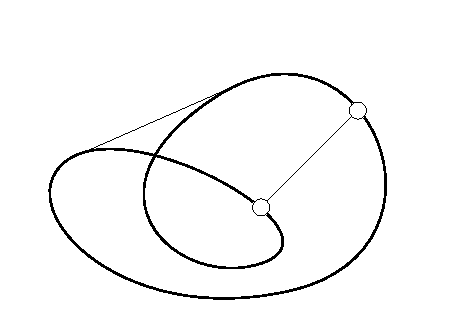
\includegraphics[scale=1,page=1]{mebius.pdf}} };
\end{tikzpicture}

\newpage
\begin{example} ($S^3$ $\mathbb{C}$  Hopf Fiber).
$S^3$ Fibration was peeoneered by Guillaume Brunerie.
\begin{lstlisting}
rot: (x : S1) -> Path S1 x x = split
    base -> loop1
    loop @ i -> constSquare S1 base loop1 @ i

mu : S1 -> equiv S1 S1 = split
    base -> idEquiv S1
    loop @ i -> equivPath S1 S1 (idEquiv S1)
                (idEquiv S1) (<j> \(x : S1) -> rot x @ j) @ i

H : S2 -> U = split
    north -> S1
    south -> S1
    merid x @ i -> ua S1 S1 (mu x) @ i

total : U = (c : S2) * H c
\end{lstlisting}
\end{example}

\begin{tikzpicture}
  \node[inner sep=20mm, fill=white, draw=black, line width=0.2mm] (img) at (0,0) {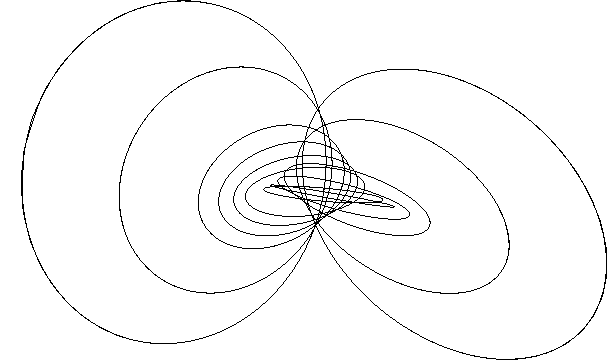
\includegraphics[scale=0.50,page=1]{hopf.pdf}};
\end{tikzpicture}

\begin{definition} (H-space).
H-space over a carrier $A$ is a tuple
$$
H_A=
\begin{cases}
A : U\\
e : A\\
\mu : A \rightarrow A \rightarrow A\\
\beta : \Pi (a:A), \mu(e,a)=a \times \mu(a,e)=a
\end{cases}
$$.
\end{definition}

\newpage
\begin{theorem} (Hopf Invariant).
Let $\phi: S^{2n-1} \rightarrow S^{n}$ a continuous map.
Then homotopy pushout (cofiber) of $\phi$ is
$cofib(\phi) = S^{n} \bigcup_\phi \mathbb{D}^{2n}$ has
ordinary cohomology
$$
H^{k}(cofib(\phi),\mathbb{Z})=
\begin{cases}
\mathbb{Z}\ for\ k=n,2n \\[2ex]
0\ otherwise
\end{cases}
$$
\end{theorem}


\begin{theorem} (Four).
There are fiber bundles:
$(S^0,S^1,p,S^1)$,
$(S^1,S^3,p,S^2)$,
$(S^3,S^7,p,S^4)$,
$(S^7,S^{15},p,S^8)$.
\end{theorem}

Hence for $\alpha,\beta$ generators of the cohomology groups in
degree $n$ and $2n$, respectively, there exists an integer $h(\phi)$
that expresses the {\textbf{cup product}} square of $\alpha$
as a multiple of $\beta$ --- $\alpha\sqcup\alpha=h(\phi)\cdot\beta$.
This integer $h(\phi)$ is called Hopf invariant of $\phi$.

\begin{theorem} (Adams, Atiyah).
Hopf Fibrations are only maps that have Hopf invariant $1$.
\end{theorem}


\bibliographystyle{plain}
\bibliography{hott}

\end{document}

